\section{Eigenschaften von reellen Funktionen}

In diesem Abschnitt wollen wir einige Eigenschaften behandeln, die eine reelle Funktion haben kann oder auch nicht. Zur Sprache kommt auch immer wieder die Frage nach Definitions- und Wertebereich einer reellen Funktion.

\subsection{Stetigkeit und Verhalten im Unendlichen}

Die meisten in Anwendungen vorkommenden Funktionen verlaufen glatt und ohne irgendwelche Sprünge. (»Die Natur kennt keine Sprünge.«) In der Mathematik nennt man solche Funktionen \textbf{stetig}.

Manchmal treten allerdings Unstetigkeiten auf, z.\,B. wird die im nächsten Beispiel vorgestellte \textbf{Sprungfunktion} in der Elektrotechnik verwendet (zur Beschreibung von Vorgängen beim Einschalten eines Stroms). Nach diesem Beispiel werden in dieser Lerneinheit nur noch stetige Funktionen vorkommen.

\subsubsection{Beispiel}

Die für alle reellen Zahlen $x \in \mathbb{R}$ erklärte \textbf{Sprungfunktion} ist an der Stelle $x_1 = 0$ unstetig. Die Sprungfunktion ist wie folgt definiert:
\begin{align*}
  f(x) &= 1 \quad \text{für } x \geq 0\\
  f(x) &= 0 \quad \text{für } x < 0
\end{align*}
Ihr Graph zeigt den Verlauf einer Stufe. Die Sprungfunktion springt an der Unstetigkeitsstelle $x_1 = 0$ von 0 auf 1. (Durch den Kreis beim Nullpunkt wird angedeutet, dass dieser Punkt \emph{nicht} zur Funktionskurve gehört, denn dort ist der Funktionswert 1.)

\begin{center}
  \begin{tikzpicture}
    \begin{axis}[width=10cm, height=4cm, axis lines=left, xmin=-5, xmax=5.3, ymin=-0.3, ymax=1.5,
      xtick={-5,...,5}, ytick={0.5,1}, xlabel={$x$}, ylabel={$y$}, tick label style={font=\footnotesize}]
      \addplot[blue, thick, domain=-5:0] {0};
      \addplot[blue, thick, domain=0:5] {1};
      \addplot[only marks, mark=o, mark size=3pt, blue, fill=white] coordinates {(0,0)};
      \addplot[only marks, mark=*, mark size=2pt, blue] coordinates {(0,1)};
    \end{axis}
  \end{tikzpicture}
\end{center}

Oft interessiert man sich dafür, wie sich eine Funktion »im Unendlichen« verhält. Damit meint man folgendes:
\begin{itemize}
  \item Was passiert mit den Funktionswerten $f(x)$, wenn $x$ immer größer wird und »gegen Unendlich strebt« (in Zeichen: $x \rightarrow \infty$)?
\end{itemize}

Zwei Beispiele sollen dies illustrieren.

\subsubsection{Beispiel}

\begin{enumerate}[label=\alph*)]
  \item Gegeben sei die Funktion $y = f(x) = x$. Die graphische Darstellung dieser Funktion (siehe das folgende Bild) ist eine Gerade.

  \begin{center}
    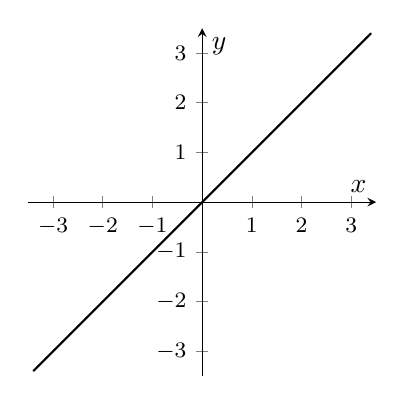
\begin{tikzpicture}
      \begin{axis}[width=6cm, height=6cm, axis lines=middle, xmin=-3.5, xmax=3.5, ymin=-3.5, ymax=3.5,
        xtick={-3,...,3}, ytick={-3,...,3}, xlabel={$x$}, ylabel={$y$}, tick label style={font=\footnotesize}]
        \addplot[black, thick, domain=-3.4:3.4] {x};
      \end{axis}
    \end{tikzpicture}
  \end{center}

  Wenn die Variable $x$ gegen Unendlich strebt ($x \rightarrow \infty$), wachsen die zugehörigen $y$-Werte der Geraden ebenfalls gegen Unendlich. Strebt $x$ gegen »Minus Unendlich« ($x \rightarrow -\infty$), so gilt dies ebenfalls für die Funktionswerte. Anschaulich bedeuten diese beiden Aussagen, dass die Funktionskurve das obige Bild nach oben rechts und nach unten links »verlässt«.

  \item Wir betrachten die Funktion $y = f(x) = \dfrac{1}{x}$ mit $x > 0$. Der Graph dieser Funktion ist eine \textbf{Hyperbel}.

  \begin{center}
    \begin{tikzpicture}
      \begin{axis}[width=6cm, height=6.5cm, axis lines=middle, xmin=-1.5, xmax=4.5, ymin=-2, ymax=4,
        xtick={-1,1,2,3,4}, ytick={-1,1,2,3}, xlabel={$x$}, ylabel={$y$}, tick label style={font=\footnotesize}, samples=200]
        \addplot[black, thick, domain=0.25:4.4] {1/x};
      \end{axis}
    \end{tikzpicture}
  \end{center}\beispielende

  Für $x \rightarrow \infty$ streben die Funktionswerte der obigen Hyperbel gegen Null. Man sagt auch: Der \textbf{Grenzwert} der Funktion für $x \rightarrow \infty$ ist gleich Null.
\end{enumerate}

\subsubsection{Beispiel}

Es wird die Funktion
\[ f(x) = \frac{x^2 + 1}{x + 1} \]
betrachtet, die für alle reellen Zahlen $x$ außer $x = -1$ definiert ist. Das folgende Bild zeigt den Graphen dieser Funktion:

\begin{center}
  \begin{tikzpicture}
    \begin{axis}[width=10cm, height=7cm, axis lines=middle, xmin=-6.2, xmax=6.3, ymin=-7.5, ymax=6,
      xtick={-6,...,6}, ytick={-6,-4,...,4}, xlabel={$x$}, ylabel={$y$}, tick label style={font=\tiny}, samples=300,
      restrict y to domain=-7.5:6]
      \addplot[black, thick, domain=-6.2:-1.05] {(x^2+1)/(x+1)};
      \addplot[black, thick, domain=-0.95:6.3] {(x^2+1)/(x+1)};
      \addplot[dashed, black, domain=-6.2:6.3] {x-1};
      \addplot[dashed, gray] coordinates {(-1,-7.5) (-1,6)};
    \end{axis}
  \end{tikzpicture}
\end{center}\beispielende

\subsubsection{Übungsaufgabe}

\begin{graukasten}
  Untersuchen Sie das Verhalten der Funktion
  \[ y = f(x) = \frac{8x^2 + 3x - 7}{4x^2 + 15} \]
  für $x \rightarrow \infty$ bzw. $x \rightarrow -\infty$. Führen Sie dazu zunächst eine Polynomdivision durch.
\end{graukasten}

\subsection{Schnittpunkte mit den Koordinatenachsen}

Aus mehreren Gründen ist es von besonderem Interesse, an welchen Stellen der Graph einer Funktion die Koordinatenachsen schneidet. Die Schnittpunkte mit der $x$-Achse nennt man \textbf{Nullstellen}. Es ist allerdings üblich, die betreffenden $x$-Werte ebenfalls als Nullstellen zu bezeichnen.

\subsubsection{Beispiel}

Die Funktion $y = f(x) = x^2 - 4$ (siehe die folgende Abbildung) schneidet die $x$-Achse in den Punkten (Nullstellen) $(2;0)$ und $(-2;0)$. Eine ebenfalls gebräuchliche Formulierung ist: Die Funktion hat die Nullstellen $x_1 = 2$ und $x_2 = -2$.

\begin{center}
  \begin{tikzpicture}
    \begin{axis}[width=9cm, height=7cm, axis lines=middle, xmin=-4.3, xmax=4.3, ymin=-4.5, ymax=12.5,
      xtick={-4,...,4}, ytick={-4,-2,...,12}, xlabel={$x$}, ylabel={$y$}, tick label style={font=\footnotesize}]
      \addplot[black, thick, domain=-3.5:3.5] {x^2-4};
    \end{axis}
  \end{tikzpicture}
\end{center}

Die Nullstellen einer Funktion $y = f(x)$ werden dadurch bestimmt, dass man $f(x_0) = 0$ setzt und diese Bestimmungsgleichung nach $x_0$ auflöst. Dieses Auflösen ist allerdings nur in einfachen Fällen rechnerisch möglich -- oft muss man raten, schätzen oder ein Computerprogramm zu Hilfe nehmen. Für die präzise Berechnung braucht man Methoden der \textbf{numerischen Mathematik}, auf die wir hier jedoch nicht eingehen können.

\subsubsection{Beispiele}

\begin{enumerate}[label=\alph*)]
  \item $y = f(x) = x^3 - x^2 + x - 1$\\
    Der Ansatz $f(x_0) = 0$ ergibt hier als einzige Lösung $x_0 = 1$.
  \item $y = f(x) = 2^x - 4$\\
    Einzige Nullstelle ist in diesem Fall $x_0 = 2$.
  \item $y = f(x) = x^6 - x - 1$\\
    Für die Nullstellen eines solchen \textbf{Polynoms sechsten Grades} gibt es keine Formel. (Darauf wurde bereits in Lerneinheit 1 hingewiesen.) Mit Hilfe eines Taschenrechners oder eines Computeralgebrasystems erhält man die beiden Lösungen $x_0 \approx 1{,}135$ und $x_0 \approx -0{,}778$.\beispielende
\end{enumerate}

Während der Graph einer Funktion die $x$-Achse mehrfach schneiden kann (im Bild zu 1.4.2.1 ist dies zweimal der Fall), kann die $y$-Achse nur einmal geschnitten werden: Gehört $x = 0$ zum Definitionsbereich der betrachteten Funktion, so markiert der an dieser Stelle angenommene Funktionswert $f(0)$ den Schnittpunkt $(0; f(0))$. Im obigen Beispiel der Funktion $y = f(x) = x^2 - 4$ ist $f(0) = -4$, d.\,h. der Schnittpunkt mit der $y$-Achse ist $(0;-4)$.

Die Schnittpunkte mit den Koordinatenachsen können in Kombination mit wenigen weiteren Überlegungen helfen, sich einen ersten Eindruck vom Verlauf einer Funktion zu verschaffen, die durch ihre Funktionsgleichung gegeben ist.

\subsubsection{Beispiel}

\begin{center}
  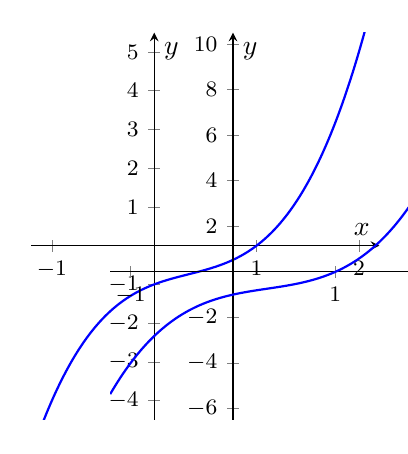
\begin{tikzpicture}
    \begin{axis}[width=6cm, height=6.5cm, axis lines=middle, xmin=-1.2, xmax=2.2, ymin=-4.5, ymax=5.5,
      xtick={-1,1,2}, ytick={-4,...,5}, xlabel={$x$}, ylabel={$y$}, tick label style={font=\footnotesize}, samples=200]
      \addplot[blue, thick, domain=-1.2:2.1] {x^3-x^2+x-1};
    \end{axis}
    \hspace{1cm}
    \begin{axis}[width=6cm, height=6.5cm, axis lines=middle, xmin=-1.2, xmax=2.2, ymin=-6.5, ymax=10.5,
      xtick={-1,1,2}, ytick={-6,-4,...,10}, xlabel={$x$}, ylabel={$y$}, tick label style={font=\footnotesize}, samples=200]
      \addplot[blue, thick, domain=-1.2:2.1] {x^3-x^2+x-1};
    \end{axis}
  \end{tikzpicture}
\end{center}

Wir schauen noch einmal auf die im vorigen Beispiel vorgekommene Funktion $y = f(x) = x^3 - x^2 + x - 1$. Da sie an der Stelle 0 den Funktionswert $-1$ hat (d.\,h. $f(0) = -1$), schneidet sie die $y$-Achse bei $y = -1$. Die $x$-Achse wird nur bei $x = 1$ geschnitten, denn dort liegt die einzige Nullstelle. Da für sehr große $x$-Werte ($x \rightarrow \infty$) auch die $y$-Werte über alle Grenzen wachsen (bzw. für $x \rightarrow -\infty$ ebenfalls beliebig ins Negative fallen), kann man bereits schließen, dass ein Schaubild der Funktion etwa so aussehen muss wie im obigen Diagramm links dargestellt. Man weiß allerdings \emph{noch nicht}, ob der Funktionsverlauf für wachsende $x$ strikt nach oben strebt wie in diesem Bild, oder ob in der Gegend von $x = 0$ die Kurve fast waagerecht verläuft bzw. sogar einmal kurz abnimmt, wie dies im rechts daneben stehenden Diagramm angedeutet ist. Diese Frage lässt sich entweder dadurch klären, dass man sich mit Computerhilfe ein Schaubild der Funktion beschafft, oder durch eine Analyse mit Hilfe der Differenzialrechnung -- dazu kommen wir erst später.\beispielende

\subsection{Weitere Eigenschaften von Funktionen}

Als nächstes wollen wir \textbf{monotone Funktionen} behandeln. Darunter versteht man Funktionen, die für wachsende $x$-Werte entweder stets steigende oder stets fallende $y$-Werte besitzen, bei denen aber nicht beides gemischt vorkommt, d.\,h. dass die $y$-Werte mal steigen, mal fallen. Am einfachsten sieht man dies an Diagrammen:

\begin{center}
  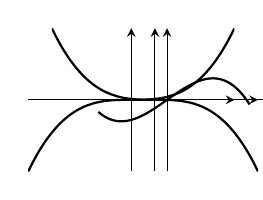
\begin{tikzpicture}
    \begin{axis}[width=4.2cm, height=3.4cm, axis lines=middle, xmin=-2, xmax=2, ymin=-2, ymax=2, xticklabels={}, yticklabels={}, xtick=\empty, ytick=\empty, samples=100]
      \addplot[thick, domain=-2:2] {x^3/4};
    \end{axis}
    \hspace{0.3cm}
    \begin{axis}[width=4.2cm, height=3.4cm, axis lines=middle, xmin=-2, xmax=2, ymin=-2, ymax=2, xticklabels={}, yticklabels={}, xtick=\empty, ytick=\empty, samples=100]
      \addplot[thick, domain=-2:2] {-x^3/4};
    \end{axis}
    \hspace{0.3cm}
    \begin{axis}[width=4.2cm, height=3.4cm, axis lines=middle, xmin=-2, xmax=2.5, ymin=-2, ymax=2, xticklabels={}, yticklabels={}, xtick=\empty, ytick=\empty, samples=100]
      \addplot[thick, domain=-1.5:1.8] {-0.3*x^3+0.9*x};
    \end{axis}
  \end{tikzpicture}
\end{center}

Die im linken Bild dargestellte Funktion ist \textbf{monoton wachsend}, die mittlere \textbf{monoton fallend}. Die rechts dargestellte Funktion ist insgesamt weder wachsend noch fallend, da sie -- wenn man wie üblich von links nach rechts die $x$-Achse »entlang läuft« -- zunächst fällt, dann wächst und schließlich wieder fällt.

Formal kann man die Monotonie folgendermaßen erklären. Das Intervall $I$ sei eine Teilmenge des Definitionsbereichs der Funktion $f$, d.\,h. es sei $I = [a,b] \subseteq D$.
\begin{itemize}
  \item $f$ heißt \textbf{streng monoton wachsend} auf $I$, wenn für beliebige $x_1, x_2 \in I$ aus $x_1 < x_2$ folgt $f(x_1) < f(x_2)$. (Wird $x$ größer, so wird $f(x)$ ebenfalls größer.)
  \item $f$ heißt \textbf{streng monoton fallend}, wenn aus $x_1 < x_2$ umgekehrt folgt $f(x_1) > f(x_2)$. (Wird $x$ größer, so wird $f(x)$ kleiner.)
  \item $f$ heißt \textbf{monoton wachsend}, wenn aus $x_1 < x_2$ folgt $f(x_1) \leq f(x_2)$. (Bei wachsendem $x$ wächst $f(x)$ oder »bleibt stehen«.)
  \item $f$ heißt \textbf{monoton fallend}, wenn aus $x_1 < x_2$ folgt $f(x_1) \geq f(x_2)$.
\end{itemize}

In allen vier Fällen heißt die Funktion $f$ \textbf{monoton} auf dem Intervall $I$.

\subsubsection{Beispiel}

Kostenfunktionen sind grundsätzlich streng monoton wachsend: Wird mehr produziert, so verursacht dies in jedem Fall höhere Gesamtkosten.\beispielende

\subsubsection{Beispiel}

Wir schauen noch einmal auf die Kostenfunktion $K(x) = 0{,}02 x^3 - 2 x^2 + 80 x + 12000$, die bereits in Beispiel 1.3.1.2 vorkam. Dividiert man hier durch $x$, so erhält man die »Kosten pro Stück« bei Produktion von $x$ Stück:
\[ \frac{K(x)}{x} = 0{,}02 x^2 - 2x + 80 + \frac{12000}{x} . \]
Dies nennt man die \textbf{Stückkostenfunktion}. Im folgenden Diagramm ist ein Graph dieser Stückkostenfunktion zu sehen:

\begin{center}
  \begin{tikzpicture}
    \begin{axis}[width=10cm, height=7cm, axis lines=left, xmin=0, xmax=210, ymin=0, ymax=1250,
      xtick={0,20,...,200}, ytick={0,200,...,1200}, xlabel={$x$}, ylabel={$K(x)/x$}, tick label style={font=\footnotesize}, samples=200,
      restrict y to domain=0:1250]
      \addplot[black, thick, domain=10:200] {0.02*x^2-2*x+80+12000/x};
    \end{axis}
  \end{tikzpicture}
\end{center}

Wie man sieht, fällt die Stückkostenfunktion zunächst auf einen Wert von ca. 200 (bei ca. $x = 90$) und steigt dann wieder an. Als Ganzes ist die Funktion weder steigend noch fallend. Interessant ist selbstverständlich der präzise $x$-Wert in der Nähe von 90, für den der kleinste Stückkostenwert angenommen wird; diesen $x$-Wert, bei dem ein \textbf{lokales Minimum} vorliegt, werden wir erst mit Hilfe der Differenzialrechnung bestimmen können (siehe später).\beispielende

\subsubsection{Übungsaufgabe}

\begin{graukasten}
  Untersuchen Sie die Funktion $y = f(x) = x^3 - 8$ hinsichtlich ihrer Schnittpunkte mit den Koordinatenachsen und ihres Unendlichkeitsverhaltens. Ist die Funktion monoton?
\end{graukasten}

\structhead{Die Umkehrfunktion}

Eine Funktion $y = f(x)$ weist jedem $x$ aus dem Definitionsbereich einen eindeutigen $y$-Wert aus dem Wertebereich zu. Dabei kann es vorkommen, dass zwei verschiedene $x$-Werte denselben $y$-Wert liefern: Beispielsweise haben $x = 2$ und $x = -2$ unter der Funktion $f(x) = x^2$ den gleichen Funktionswert. Kommt Letzteres bei einer Funktion $f$ aber \emph{nicht} vor, d.\,h. gibt es zu jedem $y$ auch immer nur einen zugehörigen $x$-Wert, der zu diesem $y$-Wert führt, so kann man jedem $y$ aus dem Wertebereich von $f$ auch das zugehörige $x$ als Funktionswert zuordnen -- man erhält so die \textbf{Umkehrfunktion} $f^{-1}$.

Die Bedeutung der Umkehrfunktion kann man sich so vorstellen, dass sozusagen die Blickperspektive gewechselt wird: Statt in den Blick zu nehmen, wie die $y$-Werte von den $x$-Werten abhängen, richtet man seine Aufmerksamkeit darauf, wie die $x$-Werte von den $y$-Werten abhängen.

Auch hier hilft erst einmal ein Beispiel.

\subsubsection{Beispiel}

Durch \textbf{Preis-Absatzfunktionen} versucht man, den Zusammenhang zwischen dem Verkaufspreis $p$ und der abgesetzten Menge $x$ eines Produkts zu beschreiben. Es ist üblich, von einer Preis-Absatzfunktion $x(p)$ zu sprechen, d.\,h. $p$ wird als die unabhängige Variable angesehen und $x$ als die abhängige. Dabei wird in der Regel $x(p)$ als streng monoton fallend angenommen -- »steigt der Preis, so sinkt der Absatz«. Eine einfache Preis-Absatzfunktion ist beispielsweise
\[ x(p) = 60 - 0{,}6\,p . \]
Im Schaubild ergibt dies eine Gerade (siehe die nächste Abbildung). Da weder ein negativer Preis relevant ist ($p < 0$) noch der Absatz negativ werden kann (ab $p > 100$), ist die Funktion nur für $p$-Werte zwischen 0 und 100 interessant.

Man kann nun auch fragen, wie umgekehrt der Preis vom Absatz abhängt, d.\,h. seinen Blick auf die Funktion $p(x)$ richten. Die zugehörige Funktionsgleichung erhält man, indem man obige Funktionsgleichung nach $p$ umstellt. Dies ergibt:
\[ p(x) = 100 - \tfrac{5}{3}\,x \]
$p(x)$ ist die Umkehrfunktion von $x(p)$.

\begin{center}
  \begin{tikzpicture}
    \begin{axis}[width=10cm, height=6.5cm, axis lines=left, xmin=0, xmax=115, ymin=-5, ymax=65,
      xtick={0,10,...,110}, ytick={0,10,...,60}, xlabel={$p$}, ylabel={$x$}, tick label style={font=\footnotesize}]
      \addplot[black, thick, domain=0:100] {60-0.6*x};
    \end{axis}
  \end{tikzpicture}
\end{center}

Wie verschafft man sich ein Schaubild der Umkehrfunktion, wenn man -- wie im obigen Beispiel -- bereits ein Schaubild der ursprünglichen Funktion vor sich hat? Man könnte sich auf den Standpunkt stellen, dies sei zugleich auch ein Schaubild der Umkehrfunktion -- wenn man darauf besteht, dass die unabhängige Veränderliche auf der waagerechten und die abhängige auf der senkrechten Achse abgebildet ist, müsste man das Diagramm eben um $90^\circ$ drehen. Üblich ist jedoch, die beiden Achsen für eine Darstellung der Umkehrfunktion zu vertauschen. In unserem Beispiel käme folgendes dabei heraus:

\begin{center}
  \begin{tikzpicture}
    \begin{axis}[width=8cm, height=6.5cm, axis lines=left, xmin=0, xmax=72, ymin=-12, ymax=105,
      xtick={0,10,...,70}, ytick={-10,0,...,100}, xlabel={$x$}, ylabel={$p$}, tick label style={font=\footnotesize}]
      \addplot[black, thick, domain=0:60] {100-5/3*x};
    \end{axis}
  \end{tikzpicture}
\end{center}

Wenn man Umkehrfunktionen von allgemeinen durch eine Funktionsgleichung $y = f(x)$ beschriebenen Funktionen betrachtet, so geht man in der Regel noch einen Schritt weiter und stellt auch die Umkehrfunktion wieder mit $x$ als unabhängiger und $y$ als abhängiger Variabler dar, man schreibt dann:
\[ y = f^{-1}(x) \]
Dies hat den Vorteil, dass dann auch die Umkehrfunktion in der üblichen Weise im $x,y$-Koordinatensystem dargestellt werden kann. Dort liegen dann die Graphen einer Funktion $f$ und der zugehörigen Umkehrfunktion $f^{-1}$ spiegelbildlich zur 1. Winkelhalbierenden, die durch die Funktionsgleichung $y = x$ gegeben ist. Für das obige Beispiel sähen dann beide Funktionen im \emph{selben} $x,y$-Koordinatensystem folgendermaßen aus:

\begin{center}
  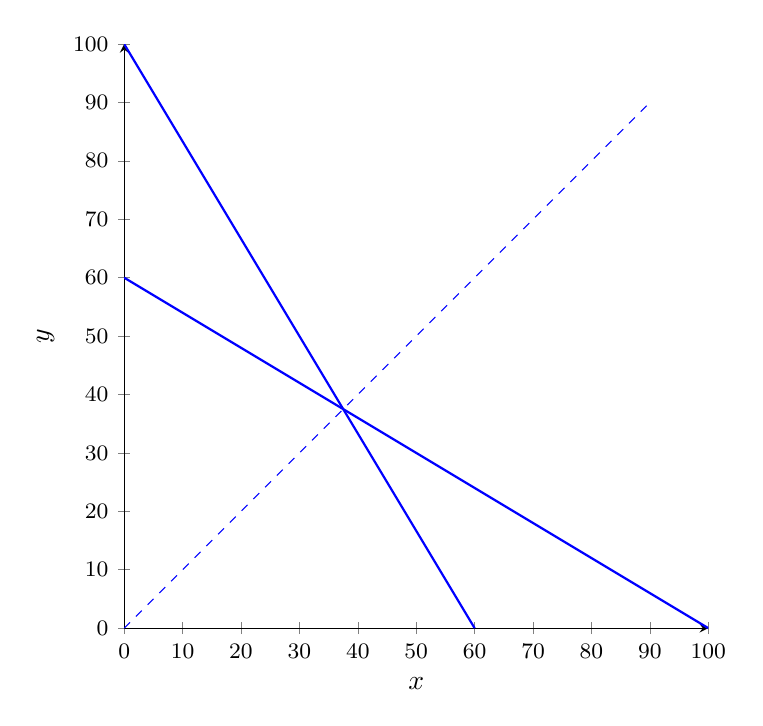
\begin{tikzpicture}
    \begin{axis}[width=9cm, height=9cm, axis lines=left, xmin=0, xmax=100, ymin=0, ymax=100,
      xtick={0,10,...,100}, ytick={0,10,...,100}, xlabel={$x$}, ylabel={$y$}, tick label style={font=\footnotesize}]
      \addplot[blue, thick, domain=0:100] {60-0.6*x};
      \addplot[blue, thick, domain=0:60] {100-5/3*x};
      \addplot[blue, dashed, domain=0:90] {x};
    \end{axis}
  \end{tikzpicture}
\end{center}

\subsubsection{Beispiel}

Wir betrachten die Funktion $y = f(x) = x^2$ nur für $x \geq 0$. Dieses $f$ ist streng monoton wachsend, die Umkehrfunktion ist
\[ y = f^{-1}(x) = +\sqrt{x} . \]
Im nächsten Schaubild sind beide Funktionen dargestellt.

\begin{center}
  \begin{tikzpicture}
    \begin{axis}[width=8cm, height=6cm, axis lines=left, xmin=0, xmax=4.3, ymin=0, ymax=4.3,
      xtick={0,1,...,4}, ytick={0,1,...,4}, xlabel={$x$}, ylabel={$y$}, tick label style={font=\footnotesize}, samples=100]
      \addplot[blue, thick, domain=0:2] {x^2};
      \addplot[blue, thick, domain=0:4] {sqrt(x)};
      \addplot[blue, dashed, domain=0:3] {x};
    \end{axis}
  \end{tikzpicture}
\end{center}\beispielende

\subsubsection{Übungsaufgabe}

\begin{graukasten}
  Bestimmen Sie zu der Funktion $y = f(x) = \tfrac{1}{2} x^3 - 1$ die Umkehrfunktion.
\end{graukasten}
